\documentclass[a5paper,10pt]{article}\usepackage[usenames,dvipsnames]{color}\usepackage{extsizes,cmap,graphicx,misccorr,indentfirst,makecell,multirow,ulem,geometry,amssymb,amsfonts,amsmath,amsthm,titlesec,float,fancyhdr,wrapfig,tikz}\usepackage[T2A]{fontenc}\usepackage[utf8x]{inputenc}\usepackage[english, russian]{babel}\usetikzlibrary{decorations.pathreplacing,decorations.pathmorphing,patterns,calc,scopes,arrows,through,positioning,shapes.misc}\graphicspath{{img/}}\linespread{1.3}\frenchspacing\geometry{left=1cm, right=1cm, top=2cm, bottom=1cm, bindingoffset=0cm}\pagestyle{fancy}\fancyhead{}\fancyhead[R]{Сарафанов Ф.Г.} 
\fancyhead[C]{Механика}
\fancyhead[L]{№109 -- Яковлев И.А.} 
\fancyfoot{}
\renewcommand{\labelenumii}{\theenumii)}
\tikzset{
	force/.style={>=latex,draw=blue,fill=blue,>=triangle 45},
    axis/.style={densely dashed,black!60,font=\small},
    interface1/.style={draw=gray!60,.
        postaction={draw=gray!60,decorate,decoration={border,angle=-135,
        amplitude=0.3cm,segment length=2mm}}},
    interface/.style={
        pattern = north east lines,
        draw    = none,
        pattern color=gray!60,          
    },
    plank/.style={
        fill=black!60, 
        draw=black,
        minimum width=3cm,
        inner ysep=0.1cm,
        outer sep=0pt,
        yshift=0.75cm,
        pattern = north east lines,
        pattern color=gray!60, 
    },
    cargo/.style={
        rectangle,
        fill=black!70,              
        inner sep=2.5mm,
    }	
}
\begin{document}

\begin{figure}[H]
    % \centering
\begin{tikzpicture}
	\def\angle{50}
	% \draw (0,2) coordinate (o) circle (2); 
	% \draw (o) circle (0.5); 
	% \draw (0,0) -- (5,6);
	\draw[interface] (0,6.25) rectangle (6,6);
	\draw[thick] (0,6) --(2.85,6) (3.15,6) --(6,6);
    \draw[interface] (0,6.25) rectangle (6,6);
    \draw [interface, draw=black]
        (2.85,6) rectangle (3.15,4);

    \def\rr{0.8}
    \draw[fill=white] (3,4) circle (\rr);
    \path (3,4) -- +(-\rr,0) coordinate (Cl) + (\rr,0) coordinate (Cr);
    \draw[fill=black] (3,4) circle (3pt);

    \draw[black!70] (Cr) -- ++ (0,-3) coordinate (B);
    \draw[black!70] (Cl) -- ++ (0,-1) coordinate (2m);

    \draw[] (B) circle (\rr);
    \path (B) -- +(-\rr,0) coordinate (Bl) + (\rr,0) coordinate (Br);
    \draw[fill=black] (B) circle (3pt);

    \draw[fill=black] (2m) rectangle ++(0.2,-0.6) rectangle ++(-0.4,0.6) node[left] {$2m$};

    \draw[black!70] (Br) -- ++ (0,-3) coordinate (o);
    \draw[black!70] (Bl) -- ++ (0,-2) coordinate (m);

    \draw[fill=black] (m) rectangle ++(0.1,-0.6) rectangle ++(-0.2,0.6) node[left] {$m$};

    \node[inner sep=0pt, scale=0.2, xshift=-2em] (russell) at (o)
    {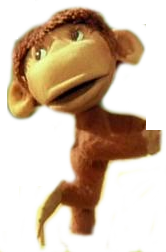
\includegraphics[width=.25\textwidth]{img/monkey.png}}; 

    \node[right, xshift=1em] at (o) {$m$};

\end{tikzpicture}
\end{figure}
\textbf{Случай $I$.} Рассмотрим движение с торможением без поворота:
\begin{equation*}
    \begin{aligned}[c]
		m\vec{a}=\vec{f}_R\\
		\text{x: }ma=-mg\mu\\
		\int_{v_0}^{v(t)}dv=\int_0^t -g\mu dt\\
		v(t)=v_0-\mu{gt}\\
		\int_{0}^{x}dx=\int_0^t [v_0-\mu{gt}] dt\\
		x(t)=v_0{t}-\mu{g}\frac{t^2}{2}
    \end{aligned}
        \qquad\qquad
    \begin{aligned}[c]
    \text{Условие остановки $v=0$ при $t=t^*$:}\\
    v_\text{ост}=0=v_0-g\mu{}t^*\\
    t^*=\frac{v_0}{g\mu}\\
    \text{Тогда пройденное до остановки $R$:}\\
    R=v_0\cdot{t^*}-\mu{g}\frac{{t^*}^2}{2}\\
    R=\frac{v_0^2}{2g\mu}
    \end{aligned}
\end{equation*}

\textbf{Случай $II$.} Поворот без торможения.
\begin{equation*}
    \begin{aligned}[c]
	m\vec{a}=\vec{f}_R\\
	v_\tau=const \Longrightarrow a_\tau=0 \\ a=a_n\\
    \end{aligned}
        \qquad\qquad
    \begin{aligned}[c]
	\text{n: } ma_n=-mg\mu\\
	\frac{v_0^2}{R}=g\mu\\
	R=\frac{v_0^2}{g\mu}
    \end{aligned}
\end{equation*}

\textbf{Вывод.} Путь до остановки с торможением без поворота  вдвое короче, чем при повороте без торможения.

\end{document}

